\documentclass[border=10pt]{standalone}
\usepackage[utf8]{inputenc}
\usepackage[romanian]{babel}
\usepackage{tikz}
\usetikzlibrary{arrows.meta,positioning,calc,fit,backgrounds}

\begin{document}
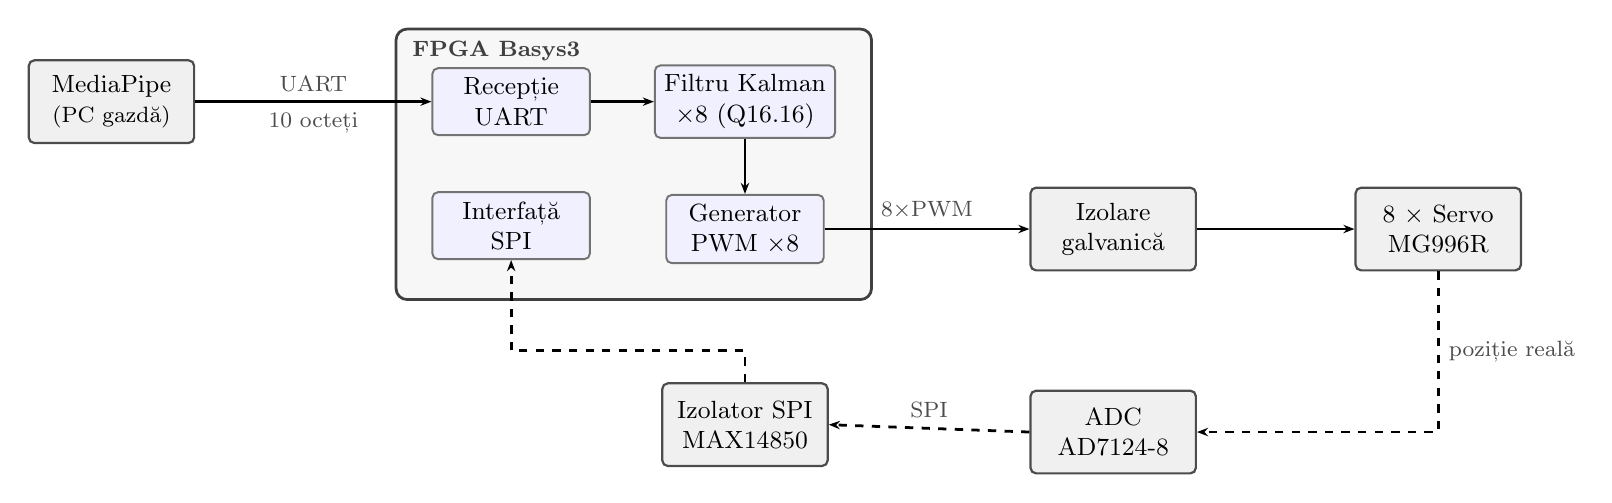
\begin{tikzpicture}[
  font=\small,
  >={Stealth[length=4pt]},
  box/.style={draw=black!70,line width=0.8pt,rounded corners=2pt,
              minimum height=1.05cm,minimum width=2.1cm,align=center,fill=white},
  ext/.style={box,fill=black!6},
  sub/.style={draw=black!55,line width=0.7pt,rounded corners=2pt,
              minimum height=0.85cm,minimum width=2.0cm,align=center,fill=blue!6},
  flow/.style={->,line width=1pt},
  lab/.style={font=\footnotesize,text=black!70}
]

% ---- blocuri externe stanga ----
\node[ext] (pc) {MediaPipe\\\footnotesize(PC gazdă)};

% ---- FPGA: containerul ----
% submodulele in interior
\node[sub,right=3.0cm of pc] (rx) {Recepție\\UART};
\node[sub,right=0.8cm of rx] (kal) {Filtru Kalman\\$\times 8$ (Q16.16)};
\node[sub,below=0.7cm of kal] (pwm) {Generator\\PWM $\times 8$};
\node[sub,below=0.7cm of rx] (spi) {Interfață\\SPI};

% conexiuni interne
\draw[flow] (rx) -- (kal);
\draw[flow] (kal) -- (pwm);

% containerul FPGA
\begin{scope}[on background layer]
  \node[draw=black!75,line width=1pt,rounded corners=4pt,fill=black!3,
        fit=(rx)(kal)(pwm)(spi),inner sep=0.45cm] (fpga) {};
\end{scope}
\node[anchor=north west,font=\footnotesize\bfseries,text=black!75]
  at ($(fpga.north west)+(0.1,-0.05)$) {FPGA Basys3};

% ---- blocuri externe dreapta ----
\node[ext,right=2.6cm of pwm] (iso) {Izolare\\galvanică};
\node[ext,right=2.0cm of iso] (servo) {8 $\times$ Servo\\MG996R};
\node[ext,below=1.5cm of iso] (adc) {ADC\\AD7124-8};
\node[ext,below=1.5cm of pwm] (isospi) {Izolator SPI\\MAX14850};

% ---- fluxul principal de semnal ----
\draw[flow] (pc) -- node[lab,above]{UART} node[lab,below]{10 octeți} (rx.west);
\draw[flow] (pwm.east) -- node[lab,above]{8$\times$PWM} (iso.west);
\draw[flow] (iso) -- (servo);

% ---- bucla de feedback (monitorizare): servo -> ADC -> izolator SPI -> FPGA ----
\draw[flow,dashed] (servo.south) |- node[lab,right,pos=0.25]{poziție reală} (adc.east);
\draw[flow,dashed] (adc.west) -- node[lab,above]{SPI} (isospi.east);
\draw[flow,dashed] (isospi.north) -- ++(0,0.4) -| (spi.south);

\end{tikzpicture}
\end{document}
